% ============================================================
%  chapter13_computational_aspects_slides.tex
%  Chapter 13: Computational Aspects
%  An Introduction to Universal Artificial Intelligence
%  Hutter, Quarel & Catt --- CRC Press, 2024
% ============================================================
\documentclass[aspectratio=169,10pt]{beamer}

\usetheme{Madrid}
\usecolortheme{seahorse}
\usefonttheme{professionalfonts}

% -- packages ------------------------------------------------------------------
\usepackage{amsmath,amssymb,bm}
\usepackage{graphicx}
\usepackage{booktabs}
\usepackage{listings}
\usepackage{xcolor}
\usepackage{tikz}
\usetikzlibrary{shapes,arrows,positioning,calc}
\usepackage{mathtools}
\usepackage{array}
\usepackage{multirow}
\usepackage{makecell}
\usepackage{stmaryrd}

\graphicspath{{figures/}}

% -- listings style --------------------------------------------------------
\lstdefinestyle{pythonstyle}{
  language=Python,
  basicstyle=\ttfamily\scriptsize,
  keywordstyle=\color{blue}\bfseries,
  stringstyle=\color{orange},
  commentstyle=\color{green!50!black}\itshape,
  numberstyle=\tiny\color{gray},
  numbers=left,
  stepnumber=1,
  numbersep=5pt,
  frame=single,
  backgroundcolor=\color{gray!7},
  breaklines=true,
  showstringspaces=false,
  tabsize=2,
  captionpos=b,
}
\lstset{style=pythonstyle}

% -- beamer setup -----------------------------------------------------------
\setbeamertemplate{footline}[frame number]
\setbeamertemplate{navigation symbols}{}
\setbeamersize{text margin left=0.5cm, text margin right=0.5cm}

% -- convenient macros -------------------------------------------------------
\newcommand{\B}{\mathbb{B}}
\newcommand{\Bstr}{\mathbb{B}^*}
\newcommand{\explain}[1]{\par\smallskip{\footnotesize\itshape #1}\par}
\newcommand{\Msol}{\mathcal{M}_{sol}}
\newcommand{\PiVA}{\Pi_{\mathrm{VA}}}
\newcommand{\Reward}{\mathcal{R}}

% -- title -------------------------------------------------------------------
\title[UAI -- Ch.13 Computational Aspects]{An Introduction to Universal Artificial Intelligence}
\subtitle{Chapter 13: Computational Aspects}
\author{Based on Hutter, Quarel \& Catt}
\institute{CRC Press, 2024}
\date{}

% =============================================================================
\begin{document}
% =============================================================================

\begin{frame}
  \titlepage
  \begin{center}
  \small\itshape ``Computing is not about computers any more. It is about living.''\\ --- Nicholas Negroponte
  \end{center}
\end{frame}

\begin{frame}{Outline}
  \tableofcontents
\end{frame}

% =============================================================================
\section{13.1 Computability of AIXI}
% =============================================================================

\begin{frame}[allowframebreaks]{Why Ask About Computability, and What We Already Know}
  The two previous chapters covered \emph{efficiently computable} approximations
  of AIXI: MDP-AIXI (Chapter 11) and MC-AIXI-CTW (Chapter 12). Both replace the
  incomputable universal mixture $\xi$ (xi) by a computable one over a
  restricted class of environments, and replace the incomputable
  \emph{expectimax} search by a feasible algorithm (dynamic programming or
  Monte Carlo Tree Search).

  \bigskip
  Clearly AIXI itself is incomputable --- but \emph{where exactly} does it sit
  in the computability hierarchy? Recall from Section 2.6.3 the
  \textbf{arithmetic hierarchy} $\Delta_n^0$ (Delta): a set or function is
  $\Delta_1^0$ iff it is ordinarily computable; it is $\Delta_2^0$
  (\emph{approximable}) iff a computable process can produce a sequence of
  guesses that eventually converges to the right answer (without ever telling
  us when it has converged); $\Delta_3^0, \Delta_4^0,\dots$ are successively
  weaker notions, each allowing one more layer of ``in the limit of a limit.''

  \bigskip
  \textbf{Goal of this chapter.} In Section 13.1 we pin down the \emph{exact}
  level of (in)computability of AIXI and several of its variants:
  \begin{itemize}
    \item \textbf{Upper bounds.} Optimal value functions, optimal policies,
      and $\varepsilon$-optimal (epsilon, ``almost optimal'') policies of AIXI
      and its variants all lie in $\Delta_n^0$ for $n=2$ or $n=3$.
    \item \textbf{Lower bounds.} None of these agents --- not even the
      weakest variant --- is computable; hence none of them is in
      $\Delta_1^0$.
  \end{itemize}
  Section 13.2 then introduces \textbf{AIXI$tl$}, a theoretically optimal
  \emph{computable} approximation of AIXI that runs in bounded time $t$ and
  uses programs of bounded length $l$ --- the price we pay is that its
  runtime is astronomically, but finitely, large.
\end{frame}

% -----------------------------------------------------------------------------
\begin{frame}[allowframebreaks]{Setting the Stage: Semimeasures, Discount, and $\Msol$}
  Before discussing the computability of \emph{optimal policies}, we first need
  the computability of \emph{value functions} (recall Section 2.6 for the
  underlying notions of computability). We focus on the class of
  \textbf{lower semicomputable environments} $\Msol$ (``sol'' for
  Solomonoff): all semimeasures that can be approximated from below by an
  algorithm.

  \begin{block}{Recap of the objects involved}
    \begin{itemize}
      \item $\nu$ (nu): a \emph{semimeasure} --- an environment model that
        assigns a (possibly sub-normalized) probability
        $\nu(e_{<t}\|a_{<t})$ to a percept history given the actions taken;
        ``semi'' because the total probability mass may be less than 1 (some
        probability can silently ``leak away'').
      \item $\gamma_k$ (gamma sub $k$): the discount weight put on the reward
        received at time $k$; $\Gamma_k$ (Gamma sub $k$), the
        \textbf{discount normalizer}, is defined so that
        $\Gamma_k := \sum_{i\ge k}\gamma_i$, which keeps values bounded in
        $[0,1]$ regardless of how many future rewards are summed.
      \item $\Reward\subset[0,1]$: the finite set of possible reward values.
      \item $V_\nu^*(h_{<t})$, $Q_\nu^*(h_{<t},a_t)$: the optimal
        (recursively defined, Theorem 6.7.2) value and Q-value functions ---
        the best expected future discounted reward achievable from history
        $h_{<t}$ (respectively, after also committing to action $a_t$).
    \end{itemize}
  \end{block}
  \explain{Solomonoff's universal mixture $\xi_U=M$ (Definition 3.7.1) is the
  most important member of $\Msol$: it is the Bayes-mixture AIXI uses as its
  ``best guess'' over \emph{all} lower semicomputable environments.}
\end{frame}

% -----------------------------------------------------------------------------
\begin{frame}{Theorem 13.1.1: Computability of $V_\nu^*$ and $Q_\nu^*$}
  \begin{block}{Theorem 13.1.1 (Computability of $V_\nu^*$ and $Q_\nu^*$)}
    Let semimeasure $\nu$, the discount normalizer $\Gamma_k$, and the
    finite reward set $\Reward\subset[0,1]$, all be $\Delta_n^0$-computable.
    Then the (recursive) optimal (Q-)value functions $V_\nu^*(h_{<t})$ and
    $Q_\nu^*(h_{<t},a_t)$ are $\Delta_n^0$-computable.
  \end{block}
  \explain{Plain English: if all the ``ingredients'' that go into defining the
  value function ($\nu$, the discounting schedule, and the possible rewards)
  can be computed to level $n$ in the arithmetic hierarchy, then the value
  function built out of them (via the Bellman-style recursion of
  Theorem 6.7.2) does not get any \emph{harder} to compute --- it stays at
  exactly the same level $n$.}

  \bigskip
  \textbf{Why this matters.} $V_\nu^*$ and $Q_\nu^*$ are the quantities an
  optimal agent needs in order to decide what to do. This theorem says:
  computing ``how good is the best possible future from here'' is no harder
  than computing the environment itself.
\end{frame}

% -----------------------------------------------------------------------------
\begin{frame}[allowframebreaks]{Remark 13.1.2 and Proof Sketch of Theorem 13.1.1}
  \begin{block}{Remark 13.1.2 (Original $V,Q$ for semimeasures can be more complex)}
    If we assume $\nu$ to be a (full) measure, then there is no difference
    between the recursive formulation (Theorem 6.7.2) and the original
    Definition 6.6.1 and Definition 6.7.1. But if $\nu$ is a genuine
    \emph{semi}measure, the definitions differ, and we explicitly have to
    take the limit $m\to\infty$ in the original definition, which pushes
    $V_\nu^*(h_{<t})$ up to $\Delta_{n+1}^0$. For finite- or moving-horizon
    agents (Definition 6.4.2) we always have $V\in\Delta_n^0$, since no
    $m\to\infty$ limit needs to be taken.
  \end{block}
  \explain{Taking a limit as $m\to\infty$ is exactly the operation that
  costs you one extra level of the arithmetic hierarchy (recall
  Section 2.6.4): $\lim \Delta_n^0 = \Delta_{n+1}^0$.}

  \framebreak

  \textbf{Proof sketch of Theorem 13.1.1.}
  \begin{enumerate}
    \item[(i)] From Theorem 6.7.2, $V_\nu^{*,m}(h_{<t})$ (the value function
      truncated to a horizon of $m$ steps) is a \emph{finite-depth}
      $(m-t)$-step recursion built from continuous combinations (sum, max,
      product, ratio) of finitely many terms, and each term is assumed
      $\Delta_n^0$. Hence $V_\nu^{*,m}(h_{<t})\in\Delta_n^0$ by
      Theorem 2.6.19 (combining finitely many $\Delta_n^0$ functions with
      computable operations keeps you in $\Delta_n^0$).
    \item[(ii)] Recall a real-valued function is \emph{computable}
      (\emph{estimable}) iff there is an algorithm that, given the input and
      any $\varepsilon>0$, computes the function to within $\varepsilon$ in
      finite time. Assume $\nu,\Gamma,\Reward\in\Delta_1^0$ (estimable).
      From Lemma 6.7.6,
      $$0\ \le\ V_\nu^*(h_{<t}) - V_\nu^{*,m}(h_{<t})\ \le\ \Gamma_{m+1}/\Gamma_t.$$
      Since $\Gamma_m\to0$ as $m\to\infty$ (Definition 6.4.1), for
      $m=t,t+1,\dots$ we estimate $\Gamma_{m+1}/\Gamma_t$ to accuracy
      $\varepsilon/4$ until we find an $m$ for which this estimate is
      $<\varepsilon/2$; for that $m$ we estimate $V_\nu^{*,m}(h_{<t})$ to
      accuracy $\varepsilon/4$. Altogether we have estimated
      $V_\nu^*(h_{<t})$ to accuracy $\varepsilon$.
    \item[(iii)] If $f(z_1,z_2,\dots)$ is computable (estimable) and
      $g_i(x_i)$ are $\Delta_n^0$-computable, then
      $f(g_1(x_1),g_2(x_2),\dots)$ is $\Delta_n^0$-computable. This lifts
      part (ii): if $\nu,\Gamma,\Reward\in\Delta_n^0$, then
      $V_\nu^*(h_{<t})\in\Delta_n^0$.
    \item[(iv)] The same argument holds for $Q_\nu^*$, which is just
      $V_\nu^*$ with the left-most $\max_{a_t}$ removed. $\blacksquare$
  \end{enumerate}
  \explain{The key trick in (ii): the proven error bound
  $\Gamma_{m+1}/\Gamma_t$ tells us exactly how deep ($m$) we must unroll the
  recursion to guarantee any desired accuracy $\varepsilon$ --- this is what
  makes $V_\nu^*$ ``estimable'' rather than merely ``defined as a limit.''}
\end{frame}

% -----------------------------------------------------------------------------
\begin{frame}[allowframebreaks]{Theorem 13.1.3: Lower Semicomputability of $V_\nu^*$, $Q_\nu^*$}
  \begin{block}{Theorem 13.1.3 (Lower semicomputability of $V_\nu^*$ and $Q_\nu^*$)}
    \begin{enumerate}
      \item[(i)] If $\nu(e_k|\cdots), \gamma_k, \Reward\in\Sigma_n^0$, then
        recursive $\Gamma_t V_\nu^*(h_{<t})\in\Sigma_n^0$.
      \item[(ii)] If $\nu(\cdots),\gamma_k,\Reward\in\Sigma_n^0$, then
        recursive $\nu(e_{<t}\|a_{<t})\Gamma_t V_\nu^*(h_{<t})\in\Sigma_n^0$.
    \end{enumerate}
  \end{block}
  \explain{$\Sigma_n^0$ (Sigma) is the ``can be confirmed from below''
  half of the arithmetic hierarchy: an approximation that only ever
  \emph{increases} towards the true value, without ever overshooting. Here
  the theorem says that if all the ingredients only ever need to be
  confirmed from below, the (rescaled) value function inherits that
  property too.}

  \textbf{Proof.} We use: if $f(z_1,z_2,\dots)$ is lower semicomputable
  ($\Sigma_1^0$) and monotone increasing in all arguments, and $g_i(x_i)$
  are $\Sigma_n^0$-computable, then $f(g_1(x_1),g_2(x_2),\dots)$ is
  $\Sigma_n^0$-computable.
  \begin{enumerate}
    \item[(i)] Inserting (6.7.3) for $\pi=\pi_\nu^{*,m}$ into (6.7.5) and
      multiplying by $\Gamma_t$ gives
      $$\Gamma_t V_\nu^{*,m}(h_{<t}) = \max_{a_t}\sum_{e_t}\nu(e_t|h_{<t}a_t)\big[\gamma_t r_t + \Gamma_{t+1}V_{\nu,\gamma}^{*,m}(h_{1:t})\big],$$
      which is $\Sigma_n^0$ since all components are $\Sigma_n^0$,
      non-negative, and combined only via $\max,\sum,\times,+$ (all
      monotone increasing), over a finite recursion. Since
      $V_\nu^{*,m}$ is monotone increasing in $m$, also
      $\Gamma_t V_\nu^{*,\infty}(h_{<t})\in\Sigma_n^0$.
    \item[(ii)] Multiplying further by $\nu(e_{<t}\|a_{<t})$,
      $$\tilde V_\nu^*(h_{<t}) := \nu(e_{<t}\|a_{<t})\Gamma_t V_\nu^*(h_{<t}) = \max_{a_t}\sum_{e_t}\big[\nu(e_{1:t}\|a_{1:t})\gamma_t r_t + \tilde V_{\nu,\gamma}^*(h_{1:t})\big],$$
      which is $\Sigma_n^0$ by the same argument. $\blacksquare$
  \end{enumerate}
\end{frame}

% -----------------------------------------------------------------------------
\begin{frame}{From Value Functions to Optimal Policies}
  These results are especially interesting for \textbf{Solomonoff's
  distribution} $\xi_U=M$, which lies in $\Msol$ (Definition 3.7.1), i.e.
  $$\xi\in\Sigma_1^0\subset\Delta_2^0.$$
  \explain{$M$ is lower semicomputable ($\Sigma_1^0$): we can always compute
  better and better lower bounds on it, we just never know exactly how close
  we currently are. Being lower semicomputable automatically implies being
  approximable ($\Delta_2^0$), one level up.}

  \bigskip
  Now that we know the level of computability of the value function, we need
  to relate it to the computability of an \emph{optimal policy} --- the
  actual decision rule the agent follows.
\end{frame}

% -----------------------------------------------------------------------------
\begin{frame}{Theorem 13.1.4: Computability of Optimal Policies}
  \begin{block}{Theorem 13.1.4 (Computability of optimal policies)}
    For any environment $\nu$, if $V_\nu^*$ is $\Delta_n^0$-computable, then
    there is an optimal (deterministic) policy $\pi_\nu^*$ for the
    environment $\nu$ that is $\Delta_{n+1}^0$-computable.
  \end{block}

  \textbf{Proof from [LH18, Thm.17].} To break ties between equally good
  actions, fix a total order $\succ$ on the action space $\mathcal{A}$
  specifying which action wins a tie. Define
  $$\pi_\nu(h_{<t}):=a \iff \bigwedge_{a':a'\succ a} Q_\nu^*(h_{<t},a)>Q_\nu^*(h_{<t},a') \ \wedge\ \bigwedge_{a':a\succ a'} Q_\nu^*(h_{<t},a)\ge Q_\nu^*(h_{<t},a').$$
  \explain{In plain English: action $a$ is chosen iff it strictly beats every
  action that is preferred to it in the tie-break order, and at least ties
  every action it is preferred over. This pins down a unique optimal action
  at every history.}

  \bigskip
  Then $\pi_\nu$ is $\nu$-optimal. Since $V_\nu^*$ is $\Delta_n^0$-computable,
  $Q_\nu^*(h_{<t},a)>Q_\nu^*(h_{<t},a')$ is $\Sigma_n^0$ and
  $Q_\nu^*(h_{<t},a)\ge Q_\nu^*(h_{<t},a')$ is $\Pi_n^0$. Therefore
  $\pi_\nu$, being a conjunction of a $\Sigma_n^0$ statement and a
  $\Pi_n^0$ statement, is itself $\Delta_{n+1}^0$. $\blacksquare$
\end{frame}

% -----------------------------------------------------------------------------
\begin{frame}{Careful! The Hierarchy Climbs Fast --- and $\varepsilon$-Optimality Saves a Level}
  This shows that if we are not careful, we quickly climb the arithmetic
  hierarchy: Solomonoff's $M\in\Delta_2^0$, which brings the iterative value
  (Definition 6.6.1) up to $\Delta_3^0$ due to the $m\to\infty$ limit,
  resulting in $\pi_M^*\in\Delta_4^0$ for \emph{infinite-horizon} AIXI.

  \bigskip
  On the other hand, Theorem 13.1.4 only states that \emph{some} optimal
  policy is $\Delta_{n+1}^0$; other optimal policies might have a strictly
  lower level. Trying to determine whether two actions have the
  \emph{exact} same value is a wasteful use of resources --- usually it is
  fine to take a slightly suboptimal action. We therefore consider policies
  guaranteed to be within $\varepsilon>0$ (epsilon) of optimal value.

  \begin{block}{Punchline}
    $\varepsilon$-optimal policies (Definition 8.1.2) require \emph{one less
    level} of computability than exactly-optimal policies.
  \end{block}
\end{frame}

% -----------------------------------------------------------------------------
\begin{frame}[allowframebreaks]{Theorem 13.1.5: Computability of $\varepsilon$-Optimal Policies}
  \begin{block}{Theorem 13.1.5 (Computability of $\varepsilon$-optimal policies)}
    For any environment $\nu$, if $V_\nu^*$ is $\Delta_n^0$-computable, then
    for all $\varepsilon>0$ there is an $\varepsilon$-optimal (deterministic)
    policy $\pi_\nu^\varepsilon$ for the environment $\nu$ that is
    $\Delta_n^0$.
  \end{block}

  \textbf{Proof from [LH18, Thm.20].} Let $\varepsilon>0$. Since $V_\nu^*$ is
  $\Delta_n^0$-computable, construct
  $Q_\varepsilon:=\{(h,a,q)\in\mathcal{H}\times\mathcal{A}\times\mathbb{Q}\mid |q-Q_\nu^*(h,a)|<\varepsilon/2\}$,
  itself $\Delta_n^0$. Fix a total tie-break order $\succ$ on
  $\mathcal{A}$. WLOG $\varepsilon=1/k$; let $Q$ be the $\varepsilon/2$-grid
  of $[0,1]$, $Q=\{0,1/2k,2/2k,\dots,1\}$. Define
  \begin{align*}
    \pi_\nu^\varepsilon(h_{<t}):=a \iff\ &\exists (q_{a'})_{a'\in\mathcal{A}}\in Q^{|\mathcal{A}|}.\ \bigwedge_{a'\in\mathcal{A}}(h,a',q)\in Q_\varepsilon\\
    &\wedge\ \bigwedge_{a':a'\succ a} q_a>q_{a'}\ \wedge\ \bigwedge_{a':a\succ a'} q_a\ge q_{a'}\\
    &\wedge\ \text{the tuple is lexicographically minimal in } Q^{|\mathcal{A}|}.
  \end{align*}
  \explain{In plain English: round every $Q$-value to the nearest point on a
  fine grid (to within $\varepsilon/2$), then pick the action with the
  highest rounded value, breaking ties lexicographically. Rounding removes
  the need to know values exactly, which is what saves a level of the
  hierarchy.}

  \bigskip
  The choice of $a$ is unique; since $\mathcal{A}$ is finite, $Q^{|\mathcal{A}|}$
  is finite too, so $\pi_\nu^\varepsilon$ is $\Delta_n^0$. $\blacksquare$
\end{frame}

% -----------------------------------------------------------------------------
\begin{frame}{Corollary 13.1.6: Putting It Together --- Computability of AIXI}
  \begin{block}{Corollary 13.1.6 (Computability of AIXI)}
    $$\pi_M^\varepsilon\in\Delta_2^0 \qquad\text{and}\qquad \pi_M^*\in\Delta_3^0.$$
    In words: there is an $\varepsilon$-optimal policy for AIXI that is
    \emph{approximable} ($\Delta_2^0$). There is an optimal AIXI policy that
    is $\Delta_3^0$.
  \end{block}
  \explain{This is the headline positive result of the chapter: although
  AIXI itself is incomputable, we now know \emph{precisely} how far up the
  arithmetic hierarchy we must go to recover it --- two levels for
  ``almost'' AIXI, three levels for exact AIXI.}
\end{frame}

% -----------------------------------------------------------------------------
\begin{frame}[allowframebreaks]{Theorem 13.1.7: No AIXI Is Computable}
  \begin{block}{Theorem 13.1.7 (No AIXI is computable)}
    (Deterministic) AIXI is incomputable, i.e. $\pi_\xi^*\notin\Delta_1^0$.
  \end{block}

  \textbf{Proof (by contradiction).} Assume $\pi_\xi^*$ is computable. Since
  it is deterministic and computable, we can build an adversarial
  environment $\mu$ (mu) that rewards the agent $0$ as long as it follows
  $\pi_\xi^*$, and rewards it $1$ forever after the \emph{first} time it
  deviates:
  $$\mu(r_t|h_{<t}a_t):=\begin{cases}
    1 & \text{if } \forall k\le t,\ a_k=\pi_\xi^*(h_{<k}) \text{ and } r_k=0\\
    1 & \text{if } \forall k\le t,\ r_k=\llbracket k\ge i\rrbracket \text{ where } i:=\min\{j\mid a_j\ne\pi_\xi^*(h_{<j})\}\\
    0 & \text{otherwise}
  \end{cases}$$
  \explain{$\llbracket\cdot\rrbracket$ is the indicator function (1 if the
  condition holds, else 0). Because $\mu$ is built \emph{from} $\pi_\xi^*$
  itself, an agent that knows and follows $\pi_\xi^*$ earns reward $0$
  forever in $\mu$ --- even though a trivially better policy (deviate once)
  would earn reward $1$ forever after.}

  \bigskip
  This gives $V_\mu^{\pi_\xi^*}(h_{<t})=0$ for all $h_{<t}$. Since $\mu$
  satisfies the conditions of Theorem 7.4.10, $V_\xi^*(h_{<t})\not\to0$ on
  histories generated by $\mu$ and $\pi_\xi^*$. But this contradicts
  Theorem 7.3.1, which guarantees
  $$V_\xi^*(h_{<t}) - V_\mu^{\pi_\xi^*}(h_{<t}) \to 0 \quad\text{for } t\to\infty,\ \mu^{\pi_\xi^*}\text{-almost surely.} \qquad\blacksquare$$
\end{frame}

% -----------------------------------------------------------------------------
\begin{frame}{Theorem 13.1.8 and Why Incomputability Is Not the End of the Story}
  \begin{block}{Theorem 13.1.8 ($\varepsilon$-AIXI is not computable)}
    $\varepsilon\text{-}AIXI\notin\Delta_1^0$.
  \end{block}
  \textbf{Proof.} See [LH18, Thm.25]. $\blacksquare$

  \bigskip
  While it is not ideal that the ``most intelligent'' general agent is
  incomputable, this is hardly surprising: it follows directly from our
  choice of what ``general'' means --- the (infinite) class of \emph{all}
  semicomputable semimeasures. Choosing \emph{smaller} classes $\mathcal{M}$
  in $\mathrm{AI}\xi$ is exactly what made MDP-AIXI and MC-AIXI-CTW
  computable (Chapters 11--12).

  \bigskip
  The primary point of AIXI was never that we expected to run it on our
  computer, but that it serves as an \textbf{ideal} --- the gold standard of
  the best possible agent we could ever hope to achieve, not the best agent
  practically achievable. The same holds for $\varepsilon$-optimal policies
  as $\varepsilon\to0$.
\end{frame}

% -----------------------------------------------------------------------------
\begin{frame}{Computability of Extensions of AIXI}
  Agents similar to AIXI, such as knowledge-seeking agents
  (Definition 9.3.2) and BayesExp (Algorithm 9.4), have similar
  computability levels.

  \begin{block}{Theorem 13.1.9 (Computability of knowledge-seeking policies)}
    For entropy-seeking and information-seeking agents, there are
    approximable ($\Delta_2^0$) $\varepsilon$-optimal policies and
    $\Delta_3^0$-computable optimal policies.
  \end{block}
  \textbf{Proof.} Follows directly from Theorems 13.1.4 and 13.1.5, letting
  the environment $\nu$ be the knowledge-seeking environment. $\blacksquare$

  \begin{block}{Theorem 13.1.10 (BayesExp is $\Delta_3^0$)}
    For any universal mixture $\xi$, BayesExp is $\Delta_3^0$.
  \end{block}

  \explain{Although $\Delta_3^0$ is far from realistically computable, the
  fact that $\varepsilon$-optimal policies are approximable ($\Delta_2^0$)
  shows we have \emph{limit-computable} algorithms for reasonably-optimal
  general agents [LH18, Thm.39].}
\end{frame}

% -----------------------------------------------------------------------------
\begin{frame}{Map: Where AIXI and Its Variants Sit in the Hierarchy}
  \begin{center}
    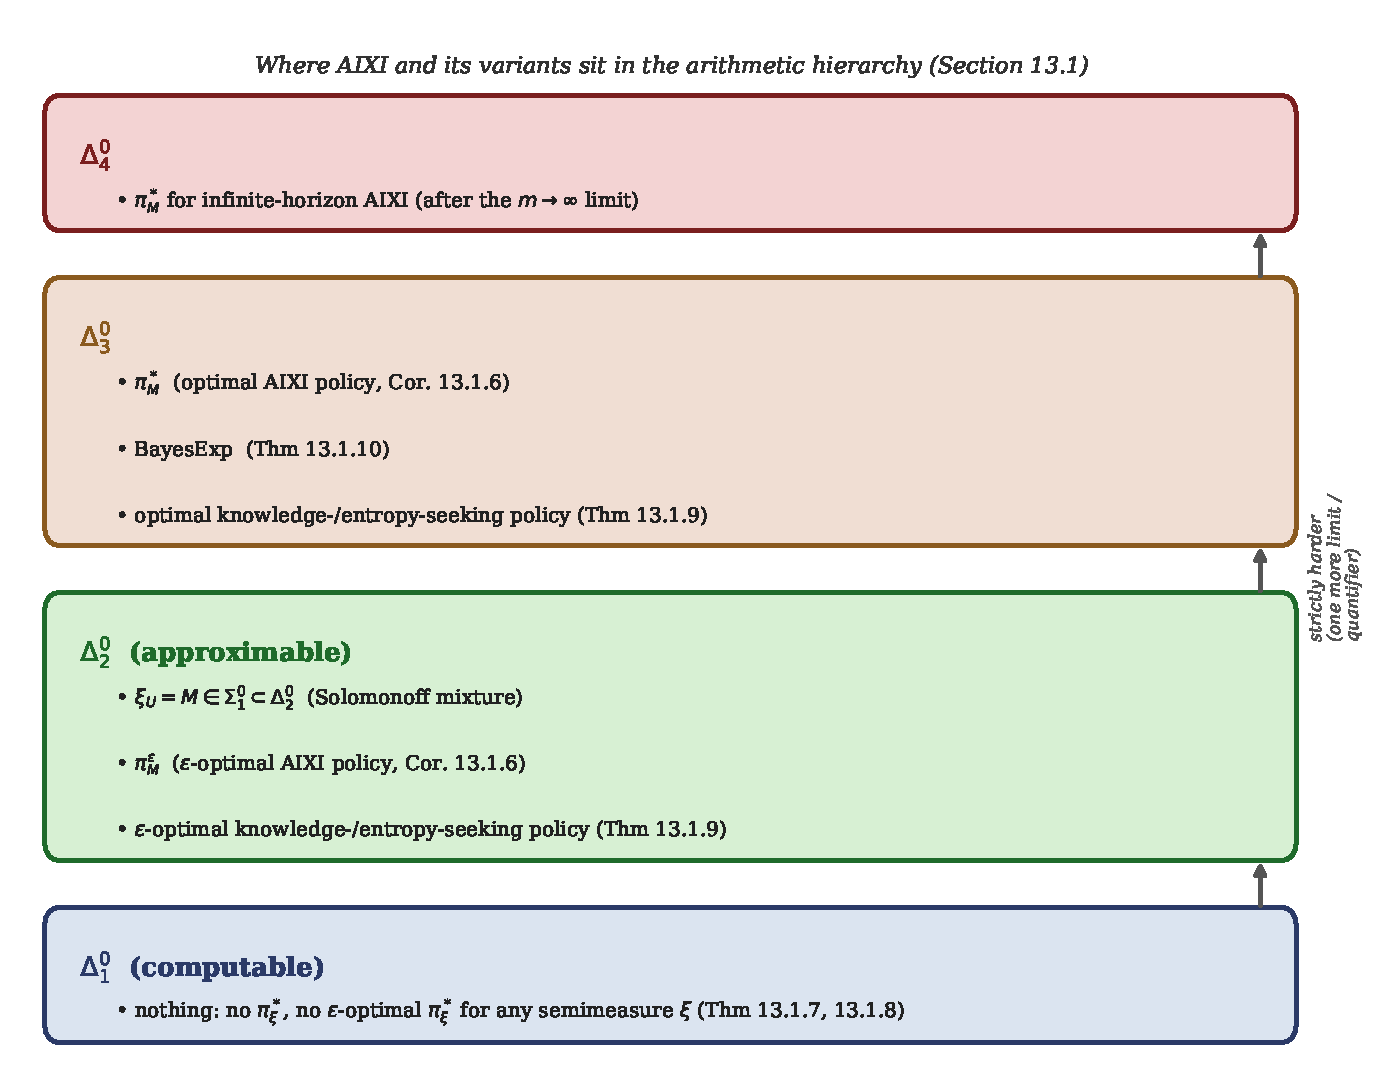
\includegraphics[width=0.78\textwidth,height=0.80\textheight,keepaspectratio]{arith_hierarchy}
  \end{center}
\end{frame}

% -----------------------------------------------------------------------------
\begin{frame}[fragile]{Python: Estimating $V_\nu^*$ via Finite-Depth Recursion}
  We make the proof of Theorem 13.1.1(ii) concrete: a toy environment with a
  \emph{constant} per-step reward $\bar r=0.7$ and geometric discounting
  $\gamma_k=\gamma^k$, $\gamma=0.9$. The recursion telescopes to
  $V_\nu^*(h_{<t})=\bar r$ exactly, while the finite-depth approximation
  $V_\nu^{*,m}(h_{<t})$ truncates the sum at depth $m$. We check numerically
  that the gap always respects the proven bound $\Gamma_{m+1}/\Gamma_t$.
\begin{lstlisting}[language=Python]
gamma, r_bar, t = 0.9, 0.7, 1
Gamma = lambda k: gamma**k / (1 - gamma)      # discount normalizer
Gt = Gamma(t)

def V_star_m(m):                              # finite-depth value, depth m
    s = sum(gamma**k * r_bar for k in range(t, m + 1))
    return s / Gt

V_true = V_star_m(100000)                      # essentially V*_nu(h<t)
for m in [1, 5, 10, 20, 40]:
    Vm    = V_star_m(m)
    bound = Gamma(m + 1) / Gt                   # proven bound Gamma_{m+1}/Gamma_t
    gap   = V_true - Vm
    print(f"m={m:3d}  V*,m={Vm:.6f}  gap={gap:.6f}  bound={bound:.6f}")
\end{lstlisting}
\end{frame}

% -----------------------------------------------------------------------------
\begin{frame}[fragile]{Python: Output --- the Gap Always Respects the Proven Bound}
\begin{lstlisting}
V*_nu(h<1) ~ 0.700000
m=  1  V*,m=0.070000  gap=0.630000  bound=0.900000
m=  5  V*,m=0.286657  gap=0.413343  bound=0.590490
m= 10  V*,m=0.455925  gap=0.244075  bound=0.348678
m= 20  V*,m=0.614896  gap=0.085104  bound=0.121577
m= 40  V*,m=0.689653  gap=0.010347  bound=0.014781
\end{lstlisting}
  \explain{The gap is always $\le$ the proven bound, and both shrink to $0$
  --- exactly the mechanism that makes $V_\nu^*$ estimable and hence
  $\Delta_n^0$ whenever $\nu,\Gamma,\Reward$ are.}
\end{frame}

% -----------------------------------------------------------------------------
\begin{frame}{Numeric Illustration of Estimability}
  \begin{center}
    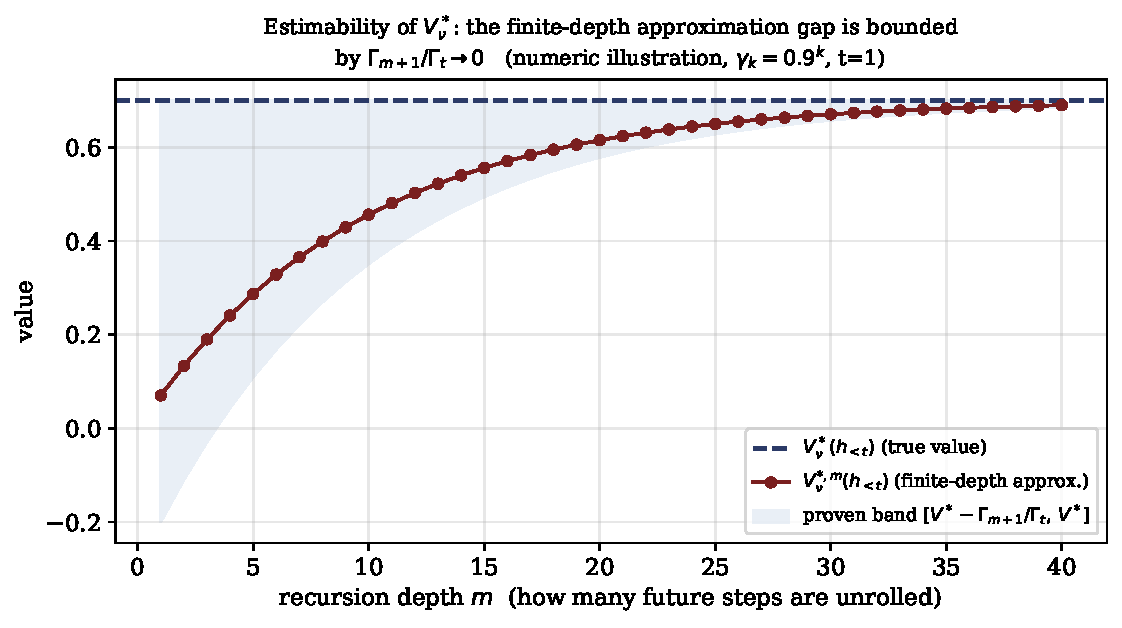
\includegraphics[width=0.78\textwidth,height=0.78\textheight,keepaspectratio]{value_convergence}
  \end{center}
\end{frame}

% =============================================================================
\section{13.2 Time- and Space-Bounded AIXI}
% =============================================================================

\begin{frame}[allowframebreaks]{Potential Approaches to Approximate AIXI}
  Knowing that AIXI is not computable, we want to know: what is the
  \emph{closest} we can get to AIXI while remaining finitely computable?

  \bigskip
  \textbf{Recap of earlier approximations.} MDP-AIXI and MC-AIXI-CTW replace
  $\xi_U$ by a computable $\xi_{\mathrm{MDP}}$ or $\xi_{\mathrm{CTW}}$, and
  replace expectimax by MCTS. Downsides:
  \begin{enumerate}
    \item[(i)] The environment class $\mathcal{M}$ is fixed \emph{a priori}
      and immutable, even if evidence suggests the true environment lies
      outside $\mathcal{M}$, or if extra compute becomes available to handle
      a larger class.
    \item[(ii)] For some problems, solving learning and planning
      \emph{jointly} is significantly more efficient than approximating
      $\xi$ and expectimax separately (e.g.\ certain Bayesian bandit
      problems have closed-form solutions).
  \end{enumerate}

  \bigskip
  \textbf{The ideal.} We want an \emph{anytime} algorithm that approaches
  AIXI in the limit of unlimited compute, and is best-in-class at every
  finite budget. This is where \textbf{AIXI$tl$} [Hut05b] comes in: it finds
  the program which, when run, leads to an agent closest to AIXI, among
  programs that halt within time $t$ and have length at most $l$.

  \framebreak

  \textbf{Why not just convert Corollary 13.1.6 into an anytime algorithm?}
  Some versions of AIXI are limit-computable (Corollary 13.1.6), so in
  principle the longer one spends (per time step) approximating the value
  function, the more accurate it becomes, converging in the limit to the
  exact value $Q_\xi^*(h_{<k},a_k)$ and $\varepsilon_k\to0$-optimal action.
  Unfortunately this is totally impractical: this algorithm converges
  \emph{slower than any computable function}.

  \bigskip
  \textbf{Another approach: fix the best policy once and for all.} Consider
  the finite class of all time- and length-bounded policies
  $\Pi_{tl}$, and determine the best-in-class policy \emph{a priori},
  $$\pi_\xi^{tl} := \arg\max_{\pi\in\Pi_{tl}} V_\xi^\pi(\epsilon),$$
  then use it for the agent's entire lifetime. Two problems:
  \begin{enumerate}
    \item[(i)] We cannot compute $\pi_\xi^{tl}$, since $V_\xi^\pi(\varepsilon)$
      is incomputable --- finding $\pi_\xi^{tl}$ is itself solving the AGI
      problem in practice.
    \item[(ii)] Fixing a \emph{single} time-bounded policy that must a priori
      handle every eventuality life throws at the agent may be wasteful.
      Finding more specialized policies the more the agent knows seems more
      promising (e.g.\ a chess engine). Note also that time-consistency no
      longer holds ($\pi_{\xi,k}^{tl}\ne\pi_{\xi,1}^{tl}$, Remark 6.6.2).
  \end{enumerate}

  \bigskip
  AIXI$tl$ addresses both problems. There are direct policy-search
  algorithms in RL that do not maintain a value function [Wil92, KHS01a],
  but these are the exception. It seems reasonable, when considering
  Bayes-optimal agents $\pi_\xi^*$, to assume the value function needs to be
  approximated well. So instead we consider an \textbf{extended policy}
  that outputs both an action \emph{and} an approximation of its own current
  value: $\dot\pi:\mathcal{H}\to\mathcal{A}\times[0,1]$. At time step $k$,
  write $a_k^{\dot\pi}=\dot\pi(h_{<k})_a$ for the action taken, and
  $v_k^{\dot\pi}=\dot\pi(h_{<k})_v$ for the claimed value estimate.

  \bigskip
  We write $\ell(\dot\pi)$ and $t(\dot\pi)$ for the \emph{length} and
  \emph{time} of an extended policy: the length of the program $p$ with
  $U(ph_{<t})=\dot\pi(h_{<t})$ for some universal Turing machine $U$, and the
  time it takes $U(ph_{<t})$ to halt. We only consider extended policies
  whose programs halt in time $\tilde t$ and have length at most $\tilde l$.
  \explain{(In this section, $k$ is used as the time index, reserving $t$ to
  denote a compute-time budget.)}
\end{frame}

% -----------------------------------------------------------------------------
\begin{frame}{Definition 13.2.1: Valid Approximation}
  Although an extended policy may take ``good'' actions, we would like to
  categorize the class of policies with ``valid'' approximations of the
  value function: those that never \emph{overrate} themselves.

  \begin{block}{Definition 13.2.1 (Valid Approximation)}
    The logical predicate $\mathrm{VA}(\dot\pi)$ is true iff $\dot\pi$ always
    satisfies $v^{\dot\pi}\le V_\xi^{\dot\pi}$, i.e.
    $$\mathrm{VA}(\dot\pi) \iff \big[\forall k\,\forall h_{<k}\in\mathcal{H}:\ \dot\pi(h_{<k})_v \le V_\xi^{\dot\pi}(h_{<k})\big].$$
  \end{block}
  \explain{In plain English: a valid extended policy may \emph{underestimate}
  its own true value $V_\xi^{\dot\pi}$, but it is never allowed to
  \emph{overclaim} --- its self-reported value estimate $v^{\dot\pi}$ must
  always be a lower bound on the value it can actually deliver.}

  \bigskip
  We only consider policies that underrate or exactly rate themselves, for
  two reasons: (i) we want to select policies with high value, but allowing
  overconfidence would let us select overrated policies whose actual value
  is much lower; (ii) combined with a lower semicomputable choice of
  $V_\xi^\pi$, this ensures AIXI$tl$ converges (in some sense) to AIXI in
  the limit $t,l\to\infty$ (Theorem 13.2.4).
\end{frame}

% -----------------------------------------------------------------------------
\begin{frame}{Definition 13.2.2: Effective Intelligence Order Relation}
  Assuming an extended policy $\dot\pi$ is a valid approximation, we want the
  ``best'' $\dot\pi$ computable with time $t$ and length $l$. This needs an
  order relation on policies based on their claimed value.

  \begin{block}{Definition 13.2.2 (Effective intelligence order relation)}
    Valid $\dot\pi$ is called \emph{effectively more or equally intelligent}
    than valid $\dot\pi'$, written $\dot\pi'\preceq_c\dot\pi$, if
    $$\dot\pi'\preceq_c\dot\pi \iff \big[\forall k\,\forall h_{<k}\in\mathcal{H}:\ \dot\pi(h_{<k})_v \le \dot\pi'(h_{<k})_v\big].$$
  \end{block}
  \explain{Careful with the direction: $\dot\pi'\preceq_c\dot\pi$ means
  $\dot\pi$'s claimed value is \emph{at least as large} as $\dot\pi'$'s at
  every history --- $\dot\pi$ claims to know a better lower bound on itself,
  so it is judged ``smarter.''}

  \bigskip
  This order relation is a \emph{self-belief} version of the (incomputable)
  total \textbf{Legg--Hutter intelligence measure} $\Upsilon(\pi)$ (Upsilon,
  Definition 16.7.1): it measures how intelligent the extended policy
  \emph{believes itself} to be, rather than how intelligent it truly is.

  \bigskip
  $\preceq_c$ is an \textbf{upper semicomputable partial order} on extended
  policies: it is reflexive, antisymmetric, and transitive, and (as a
  function) upper semicomputable. Without resource restrictions, it would
  still have a global maximum $\dot\pi\preceq_c\dot\pi_\xi^*:=(\pi_\xi^*,V_\xi^*)$
  for all valid $\dot\pi$.
\end{frame}

% -----------------------------------------------------------------------------
\begin{frame}[allowframebreaks]{The AIXI$tl$ Algorithm --- Setup Phase}
  AIXI$tl$ takes as inputs a max time $\tilde t$, a max length $\tilde l$,
  and a max proof length $l_P$ (used for the maximum length of correctness
  proofs).

  \bigskip
  \textbf{Setup (before interaction begins).} Check through all
  $b\in\B^{l_P}$ in some order, testing whether $b$ constitutes a
  \emph{proof} that some $\dot\pi$ of length at most $\tilde l$ is a valid
  extended policy. ``Proof'' means: $b$ is interpreted as a proof in the
  same formal axiomatic system in which $\mathrm{VA}(\cdot)$ is defined.
  Every recorded pair $(b,\dot\pi)$ contributes $\dot\pi$ to the set
  $\Pi_{\mathrm{VA}}$ of all such proven-valid policies.

  \bigskip
  \explain{This setup takes $O(l_P^2\,2^{l_P})$ time: checking $2^{l_P}$
  candidate proofs, each in time $O(l_P^2)$. Crucially, this cost is
  \emph{unrelated} to $\tilde t$ --- it only depends on the proof-search
  budget $l_P$. It requires significant compute, and some justification for
  why a voting-style algorithm over machine-checked proofs is an
  unavoidable ingredient.}

  \framebreak

  We then modify every $\dot\pi\in\Pi_{\mathrm{VA}}$ so that, during any
  cycle $k$, if $\dot\pi$ does not halt within time $\tilde t$, it is forced
  to output $(a,0)$ for an arbitrary $a$ --- claiming value $0$, which is
  automatically valid. This guarantees every $\dot\pi\in\Pi_{\mathrm{VA}}$
  runs in time at most $\tilde t$ and remains valid.
\end{frame}

% -----------------------------------------------------------------------------
\begin{frame}[fragile]{Algorithm 13.1: AIXI$tl$}
\begin{lstlisting}[language=Python, basicstyle=\ttfamily\scriptsize, morekeywords={Require,Input,Output,for,do,Set,Choose,Write,Receive}]
Algorithm 13.1  AIXItl [Hut05b]
Require: Max time t~, max program length l~, max proof length l_P
Input:   Percept stream e1, e2, e3, ...
Output:  (t~, l~, l_P)-optimal action stream a1, a2, a3, ...

 1: Interpret all b in B^{l_P} as proofs of VA(pi-dot) for some pi-dot
 2: Let Pi_VA be the set of those pi-dot's such that
      length(pi-dot) <= l~  and  VA(pi-dot) has been proven
 3: Modify each pi-dot so that, in cycle k, if it does not output
      (a_k, v_k^{pi-dot}) within time t~, force it to output (a, 0)
 4: Update Pi_VA to be the set of these new pi-dot's
 5: Set k := 1
 6: for k = 1, 2, 3, ... do
 7:     for pi-dot in Pi_VA do
             run pi-dot on h_{<k}; receive pi-dot(h_{<k}) = (a_k^{pi-dot}, v_k^{pi-dot})
 8:     Choose pi-dot* = argmax_{pi-dot in Pi_VA} v_k^{pi-dot}   (highest claimed value)
 9:     Write a_k := a_k^{pi-dot*}  on the output tape
10:     Receive input e_k from the environment
\end{lstlisting}
  \explain{Every cycle, AIXI$tl$ runs \emph{every} proven-valid extended
  policy on the current history, and simply acts according to whichever one
  currently \emph{claims} the highest value. Because every $\dot\pi$ in
  $\Pi_{\mathrm{VA}}$ is provably valid (never overrates itself), trusting
  the loudest claim is provably safe.}
\end{frame}

% -----------------------------------------------------------------------------
\begin{frame}[allowframebreaks]{AIXI$tl$: Why Trusting the Highest Claim Works}
  Since every $\dot\pi\in\Pi_{\mathrm{VA}}$ has a proof of
  $\mathrm{VA}(\dot\pi)$, we know that for all $k$,
  $$v_k^{\dot\pi} \le V_\xi^{\dot\pi}(h_{<k}).$$
  This means picking the $\dot\pi$ with the largest $v_k^{\dot\pi}$ leads to
  the most intelligent agent according to the effective intelligence order
  relation $\preceq_c$. Additionally, since at each interaction cycle we
  loop through $\Pi_{\mathrm{VA}}$, whose \emph{size} is independent of
  $\tilde t$, each cycle takes time $O(\tilde t)$ per policy evaluated ---
  i.e.\ the same $\tilde t$ budget, repeated $|\Pi_{\mathrm{VA}}|$ times.

  \begin{block}{Theorem 13.2.3 (Optimality of AIXI$tl$ [Hut05b])}
    Let $\dot\pi$ be any extended policy of length $\ell(\dot\pi)\le\tilde l$
    and computation per cycle $t(\dot\pi)\le\tilde t$, for which there
    exists a proof of $\mathrm{VA}(\dot\pi)$ of length $\le l_P$.
    Algorithm 13.1, which depends on $\tilde l,\tilde t,l_P$ but \emph{not}
    on $\dot\pi$, is effectively more or equally intelligent according to
    $\preceq_c$ than any such $\dot\pi$.

    \medskip
    The length of the optimal policy found, $\dot\pi^*$, is
    $\ell(\dot\pi^*)=O(\log(\tilde l\cdot\tilde t\cdot l_P))$; the setup
    time is $t_{\mathrm{setup}}(\dot\pi^*)=O(l_P^2\,2^{l_P})$; and the
    computation time per cycle is
    $t_{\mathrm{cycle}}(\dot\pi^*)=O(2^{\tilde l}\cdot\tilde t)$.
  \end{block}

  \textbf{Proof.} A direct consequence of the construction: at each time
  step, if $\dot\pi$ is the most effectively intelligent policy in
  $\Pi_{\mathrm{VA}}$, AIXI$tl$ acts according to it; if not, AIXI$tl$ acts
  as the more effectively intelligent policy would. Either way, AIXI$tl$ is
  effectively more or equally intelligent according to $\preceq_c$.
  $\blacksquare$

  \explain{Note: potentially following a \emph{different} policy at each
  time step might seem counterintuitive, but it does not matter for
  AIXI$tl$, whose only objective is to maximize its effective intelligence
  at each individual step, using whatever is available in $\Pi_{\mathrm{VA}}$
  at that moment.}
\end{frame}

% -----------------------------------------------------------------------------
\begin{frame}{The AIXI$tl$ Interaction Loop, Visualized}
  \begin{center}
    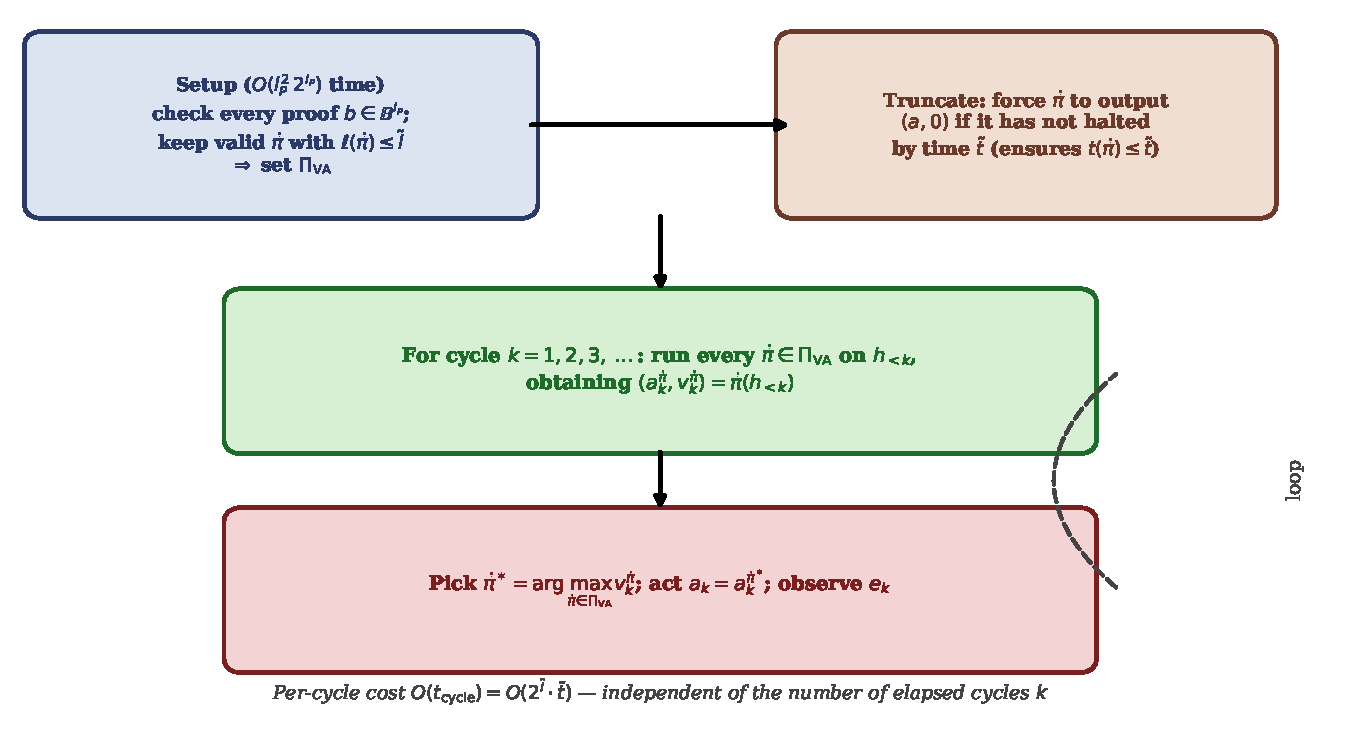
\includegraphics[width=0.88\textwidth,height=0.80\textheight,keepaspectratio]{aixitl_loop}
  \end{center}
\end{frame}

% -----------------------------------------------------------------------------
\begin{frame}{Just How Impractical? And Does AIXI$tl$ Approach AIXI?}
  Although the setup time and time per cycle are rather large, if we fix
  $l_P$ and $\tilde l$, the setup time is \emph{constant} in $\tilde t$ and
  the time per cycle is $O(\tilde t)$ --- although these hidden constants
  are extremely (astronomically) large in practice.

  \bigskip
  \textbf{Does AIXI$tl$ approach AIXI as the budgets grow?} A key
  requirement is that $V_\xi^*(h_{<k})$ be lower semicomputable.
  Theorem 13.1.3 gives two routes (for $n=1$): (i) we would need
  $\xi(e_k|h_{<k}a_k)$ itself lower semicomputable --- but $\xi\in\Msol$ does
  \emph{not} satisfy this (a construction similar to Section 10.5 may still
  work); (ii) we only need the \emph{joint}
  $\xi(e_{<t}\|a_{<t})$ lower semicomputable, which \emph{does} hold for
  $\xi=\xi_U$. This gives us
  $\tilde V_{\xi_U}^*(h_{<t}):=\xi_U(e_{<t}\|a_{<t})\Gamma_t V_{\xi_U}^*(h_{<t})$,
  lower semicomputable, which can replace $V_\xi^*$ in Definition 13.2.1
  without affecting the effective intelligence order relation (both
  $\dot\pi$'s are scaled by the same factor, independent of $a_t$).

  \begin{block}{Theorem 13.2.4 (AIXI$tl$ approaches AIXI)}
    If the scaled optimal value function $\tilde V_\xi^*(h_{<k})$ is used and
    is lower semicomputable, then the behavior of AIXI$\tilde t\tilde l$
    approaches the behavior of AIXI in the limit
    $\tilde t,\tilde l,l_P\to\infty$, in some sense.
  \end{block}
\end{frame}

% -----------------------------------------------------------------------------
\begin{frame}[allowframebreaks]{Proof Sketch of Theorem 13.2.4, and Conclusion}
  \textbf{Proof sketch.} Lower semicomputability of $V_\xi^*(h_{<k})$
  ensures the existence of a sequence of extended programs
  $\dot\pi_1,\dot\pi_2,\dot\pi_3,\dots$ for which $\mathrm{VA}(\dot\pi_i)$
  can be proven and $\lim_{i\to\infty} v_k^{\dot\pi_i}=V_\xi^*(h_{<k})$ for
  all $k$ and histories $h_{<k}$. One such sequence: terminate some
  (non-halting) lower-semicomputing scheme for $Q_\xi^*(h_{<k},a_k)$ after
  $i$ time steps, and use the obtained approximation as $v_k^{\dot\pi_i}$
  for the action $a_k^{\dot\pi_i}$ maximizing the approximate Q-value. The
  convergence $v_k^{\dot\pi_i}\to V_\xi^*(h_{<k})$ ensures that the
  universally optimal value can be approximated by \emph{some} provably
  valid $\dot\pi$ arbitrarily well, given enough time and length. The
  approximation is not uniform in $k$, but this does not matter, as the
  selected $\dot\pi$ is allowed to change from interaction cycle to cycle.
  $\blacksquare$

  \begin{block}{Conclusion}
    Similar to other reinforcement learning algorithms, AIXI$tl$ evaluates
    policies, but in an unusual, \textbf{provably pessimistic} way: it
    insists on a proof of correctness (valid approximation) before
    comparing a policy to every other valid, non-overconfident policy.
    Crucially, AIXI$tl$ does not require $\dot\pi$ to first estimate a model
    $\xi_U$ and then compute $V_{\xi_U}^*$ separately --- it can estimate the
    latter directly, model-free, or in whatever way is most efficient. While
    dovetailing through all programs to find the best is a well-known idea,
    making it work for AIXI was non-trivial, since $V_{\xi_U}^*$ itself is
    incomputable; lower semicomputability of the scaled
    $\tilde V_{\xi_U}^*$ was crucial. Roughly: if some unknown policy $\pi$
    of size $\tilde l$ and per-cycle time $\tilde t$ has certain
    capabilities (chess master, AGI, ASI), then the known, computable
    AIXI$\tilde t\tilde l$ has the same capabilities within the same time
    frame, up to an (unfortunately very large) constant factor.
  \end{block}
\end{frame}

% -----------------------------------------------------------------------------
\begin{frame}{Why AIXI$tl$ Is Optimal but Utterly Impractical}
  \begin{center}
    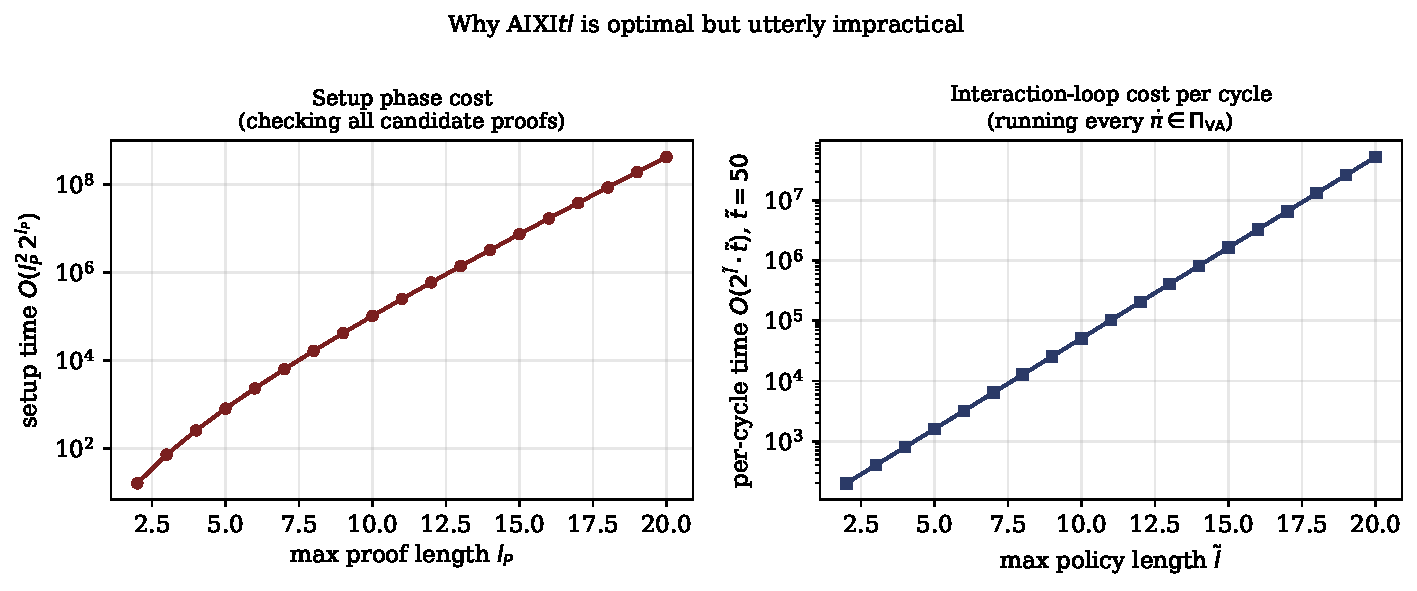
\includegraphics[width=0.88\textwidth,height=0.78\textheight,keepaspectratio]{search_cost}
  \end{center}
\end{frame}

% -----------------------------------------------------------------------------
\begin{frame}[fragile]{Python: A Toy Universal Search over $\Pi_{\mathrm{VA}}$}
  A miniature illustration of the mechanism at the heart of AIXI$tl$: we
  enumerate every candidate ``extended policy'' as a bit-string of length
  $\le \tilde l$ (a stand-in for the finitely many proven-valid programs in
  $\Pi_{\mathrm{VA}}$), let each one output a deterministic ``self-claimed
  value'' $v^{\dot\pi}$, and pick the $\arg\max$ --- exactly line~8 of
  Algorithm 13.1.
\begin{lstlisting}[language=Python]
import itertools

def claimed_value(bits):                     # toy deterministic self-rating
    h = sum((i + 1) * int(b) for i, b in enumerate(bits))
    return (h % 97) / 97                       # a pseudo-value in [0,1)

l_tilde = 4                                    # max program length
candidates = [''.join(bits)
              for length in range(l_tilde + 1)
              for bits in itertools.product('01', repeat=length)]
print(f"|Pi_VA| = {len(candidates)} candidates of length <= {l_tilde}")

scored = sorted(((pi, claimed_value(pi)) for pi in candidates),
                 key=lambda x: -x[1])
for pi, v in scored[:5]:
    print(f"  pi_dot={pi or '(empty)':>6s}   v={v:.4f}")

best_pi, best_v = scored[0]
print(f"AIXItl acts as pi_dot* = {best_pi!r}, claimed value {best_v:.4f}")
\end{lstlisting}
\end{frame}

% -----------------------------------------------------------------------------
\begin{frame}[fragile]{Python: Output --- Picking the Highest Claimed Value}
\begin{lstlisting}
|Pi_VA| = 31 candidates of length <= 4
  pi_dot=  1111   v=0.1031
  pi_dot=  0111   v=0.0928
  pi_dot=  1011   v=0.0825
  pi_dot=  0011   v=0.0722
  pi_dot=  1101   v=0.0722
AIXItl acts as pi_dot* = '1111', claimed value 0.1031
\end{lstlisting}
  \explain{With $\tilde l=4$ there are already $31=2^5-1$ candidates; the
  \texttt{search\_cost} figure shows this count exploding as $O(2^{\tilde l})$
  --- exactly why the theorem's constants are astronomically large.}
\end{frame}

% =============================================================================
\section{13.3 Exercises}
% =============================================================================

\begin{frame}[allowframebreaks]{13.3 Exercises}
  \begin{enumerate}
    \item[1.] [C30] Prove (or disprove): for any environment $\nu$, if
      $V_\nu^*$ is $\Delta_n^0$-computable, then there exists an optimal
      (deterministic) policy $\pi_\nu^*$ for the environment $\nu$ that is
      \emph{not} $\Delta_n^0$-computable.

    \item[2.] [C32] Prove (or disprove): for any environment $\nu$, if
      $V_\nu^*$ is $\Delta_n^0$-computable, then for $\varepsilon>0$ there is
      \emph{no} $\varepsilon$-optimal (deterministic) policy
      $\pi_\nu^\varepsilon$ for the environment $\nu$ that is
      $\Delta_{n-1}^0$.

    \item[3.] [C22] Prove Corollary 13.1.6.

    \item[4.] [C26] Prove Theorem 13.1.8, that $\varepsilon$-AIXI is not
      computable.

    \item[5.] [C40] Various results of this chapter assumed deterministic
      policies. Prove (or disprove) that they also hold for stochastic
      policies.

    \item[6.] [C26] Prove that BayesExp is $\Delta_3^0$.

    \item[7.] [C40] Derive the computability bounds for Thompson sampling.
  \end{enumerate}
  \explain{The bracketed numbers such as [C30] are the book's difficulty
  ratings for each exercise (roughly, ``C'' for a problem requiring
  creative/compositional reasoning, with the number indicating relative
  difficulty/length).}
\end{frame}

% =============================================================================
\section{13.4 History and References}
% =============================================================================

\begin{frame}[allowframebreaks]{13.4 History and References}
  \textbf{Computability in RL.} This chapter is based on material from
  [LH18] and [Lei16b, Chp.\,6]. Many results around the computability of
  AIXI and other UAI agents were first derived in [LH15c, LH15d] and later
  extended in [Lei16b, LH18]. While this is the first work showing
  computability results in the UAI framework, traditional RL has many
  computability and complexity-theory results of its own. On the
  complexity-theory side, planning is P-complete in MDPs with finite and
  infinite horizons [PT87]. [MGLA00] proved (among other results) that
  deciding whether a sufficiently good policy exists in MDPs and POMDPs is
  PSPACE-complete. [LGM01] showed that (unless the polynomial hierarchy
  collapses, e.g.\ P$=$NP) optimal policies for MDPs and POMDPs are not
  $\varepsilon$-approximable. [SLR07] showed that deciding whether there
  exists a policy with value exceeding a given value in epistemic POMDPs is
  PSPACE-complete, as well as the existence of an optimal policy in an
  epistemic POMDP being NP. On the computability side, [MHC99, MHC03] showed
  that planning with infinite horizon in general POMDPs is even formally
  undecidable.

  \bigskip
  On the topic of Solomonoff induction, [Net22] argued that the problems of
  the relative choice of machine and incomputability in Solomonoff
  prediction are both caused by the fact that computable approximations of
  Solomonoff prediction do not always converge.

  \bigskip
  Regarding halting and termination of programs, [Ica17] showed that when
  using probabilistic computation in cognitive science, it is not always
  desirable to have models which always terminate, and argues for some
  benefits of non-terminating models.

  \framebreak

  \textbf{AIXI$tl$.} AIXI$tl$ (Section 13.2) was first introduced in
  [Hut00] and described again in [Hut03d, Hut05b, Hut07f, Hut12b, Lei16b].
  [Pan08] developed a more practical approximation based on Monte Carlo Tree
  Search sampling programs. Further replacing the Solomonoff prior by CTW
  led to MC-AIXI-CTW (Chapter 12). [Kat18] introduced a more functional
  approximation based on typed lambda calculus and argued it to be even
  more powerful than AIXI$tl$.
\end{frame}

% -----------------------------------------------------------------------------
\begin{frame}[allowframebreaks]{13.4 History and References (cont'd): Optimal Solvers and Universal Search}
  One key component of AIXI$tl$ is that of \textbf{universal (Levin) search}.
  Introduced in [Lev73c], universal search is a method designed to
  efficiently find a program that can solve a problem, provided the
  solution can be efficiently verified.

  \bigskip
  There have been many extensions of Universal Search:
  \begin{itemize}
    \item An adaptive extension of Levin Search was introduced in [WS96],
      used to solve POMDPs.
    \item {[Hut01b, Hut02b]} extends Levin search to a provably fastest
      algorithm for all well-defined problems, even if the solution cannot
      be verified efficiently.
    \item {[Sch04]} develops a more practical Adaptive version of Levin
      Search (ALS), called the \textbf{Optimal Ordered Problem Solver}
      (OOPS), which can take advantage of previous solutions.
    \item \textbf{Levin Tree Search} (LTS) [OLLW18] is a policy-guided
      search algorithm with an adaptive policy that comes with theoretical
      guarantees. The policy may be represented using neural networks
      (LTS+NN) [OL21], or parameterized in a convex way using context
      models (LTS-CM) [OHL23], with theoretical guarantees and
      award-winning practical performance on Sokoban, The Witness, and the
      24-Sliding Tile puzzle.
  \end{itemize}

  \bigskip
  Also related to Universal Search is the \textbf{G\"odel Machine}
  [Sch07], a formal self-improving optimal problem solver. [Sch05] argued
  how the G\"odel Machine could be used for a formal definition of
  consciousness. Several potential implementations of the G\"odel Machine
  are discussed in [SS11].
\end{frame}

% =============================================================================
\end{document}
